\section{Introdução}\label{introduuxe7uxe3o}

Este trabalho aborda três formas de comunicação de dados em aplicações
desenvolvidas com MPI, comparando seu desempenho. Os modelos de
comunicação analisados são os seguintes:

\begin{enumerate}
\tightlist
\item
  \textbf{Comunicação coletiva:} utiliza operações coletivas do MPI,
  empregando MPI\textsubscript{Scatter} para distribuir as linhas da
  matriz (A), MPI\textsubscript{Bcast} para difundir a matriz (B) e
  MPI\textsubscript{Gather} para reunir a matriz resultante. Nessa
  abordagem, a biblioteca MPI decide internamente a estratégia mais
  eficiente para realizar a comunicação entre os processos.
\item
  \textbf{Comunicação ponto a ponto bloqueante (síncrona):} o processo
  mestre envia cada parcela dos dados utilizando
  MPI\textsubscript{Send}, enquanto os processos trabalhadores as
  recebem por meio de MPI\textsubscript{Recv}. Cada operação retorna
  apenas após a conclusão da transferência correspondente. A matriz (B)
  continua sendo distribuída com MPI\textsubscript{Bcast}.
\item
  \textbf{Comunicação ponto a ponto não bloqueante (assíncrona):}
  utiliza MPI\textsubscript{Isend}, MPI\textsubscript{Irecv} e
  MPI\textsubscript{Ibcast}, que apenas iniciam as operações de
  comunicação e retornam imediatamente. A sincronização ocorre
  posteriormente por meio de MPI\textsubscript{Wait}, garantindo a
  conclusão das transferências antes da utilização dos dados.
\end{enumerate}

O problema escolhido para a comparação foi a multiplicação de duas
matrizes de dimensão (N × N). Nessa aplicação, o processo de rank 0
(mestre) divide as linhas da matriz (A) entre todos os processos,
distribui a matriz (B) integralmente para cada um deles, cada processo
calcula sua respectiva parcela da matriz resultante e, ao final, devolve
o resultado ao processo mestre.

\section{Metodologia}\label{metodologia}

Os experimentos rodaram na partição \texttt{hype} do cluster PCAD (nós
com 2x Xeon E5-2650 v3, 20 núcleos físicos por nó), com MPI sobre TCP e
sem fixação de processos a núcleos (\texttt{-\/-bind-to\ none}). Todas
as combinações dos fatores abaixo foram executadas 2 vezes (324
execuções no total):

\begin{longtable}[]{@{}ll@{}}
\toprule\noalign{}
Fator & Níveis \\
\midrule\noalign{}
\endhead
\bottomrule\noalign{}
\endlastfoot
Tipo comunicação & coletiva, p2p bloqueante, p2p não bloqueante \\
Nós & 1, 2, 3 \\
Processos por nó & 1, 2, 4, 8, 16, 32 \\
Tamanho (NxN) & 500, 1000, 1500 \\
\end{longtable}

Cada execução foi rastreada com a biblioteca akypuera: toda chamada MPI
de todo processo fica registrada com início, fim e duração. As análises
foram feitas a partir desses rastros. As métricas usadas são:

\begin{itemize}
\tightlist
\item
  \textbf{Tempo total}: medido pela própria aplicação com
  \texttt{MPI\_Wtime} no processo 0 (do início da distribuição até o fim
  da coleta).
\item
  \textbf{Tempo por função MPI}: para uma execução, somamos quanto cada
  processo passou dentro de cada função (por exemplo, todo o tempo de
  \texttt{MPI\_Recv} do processo 3) e tiramos a média entre os
  processos. Isso responde: "em média, quanto um processo gasta nessa
  função?"
\item
  Como cada configuração rodou 2 vezes, reportamos a mediana das duas e
  usamos o desvio padrão como indicação de variabilidade.
\end{itemize}

\texttt{MPI\_Finalize} é excluído do tempo por função: ele só marca o
fim do programa, e sua duração é apenas espera pelos processos mais
lentos.

Duas limitações do código, iguais nas três versões: a divisão de linhas
usa divisão inteira (\texttt{n/size}), então quando N não é múltiplo do
número de processos as últimas linhas não são calculadas; e, na versão
não bloqueante, o mestre nunca espera seus próprios \texttt{Isend}
terminarem, o que o padrão MPI não permite (aqui funciona, mas é
incorreto).

\section{Linha do tempo das execuções
(Gantt)}\label{linha-do-tempo-das-execuuxe7uxf5es-gantt}

A forma mais direta de ver a diferença entre as versões é desenhar a
linha do tempo de uma execução: cada linha horizontal é um processo e o
tempo corre para a direita. Trechos coloridos são chamadas MPI (uma cor
por função); trechos em branco são computação (o processo está
multiplicando matrizes, sem comunicar); o cinza final é o
\texttt{MPI\_Finalize} (o processo já acabou e está esperando os
demais).

Usamos a maior configuração do experimento -- matriz 1500x1500, 96
processos em 3 nós (32 por nó) -- porque é onde a comunicação mais
aparece. Os processos 0 a 31 estão no mesmo nó que o mestre; os demais
estão em nós remotos, acessados pela rede.

\begin{figure}[H]
\centering
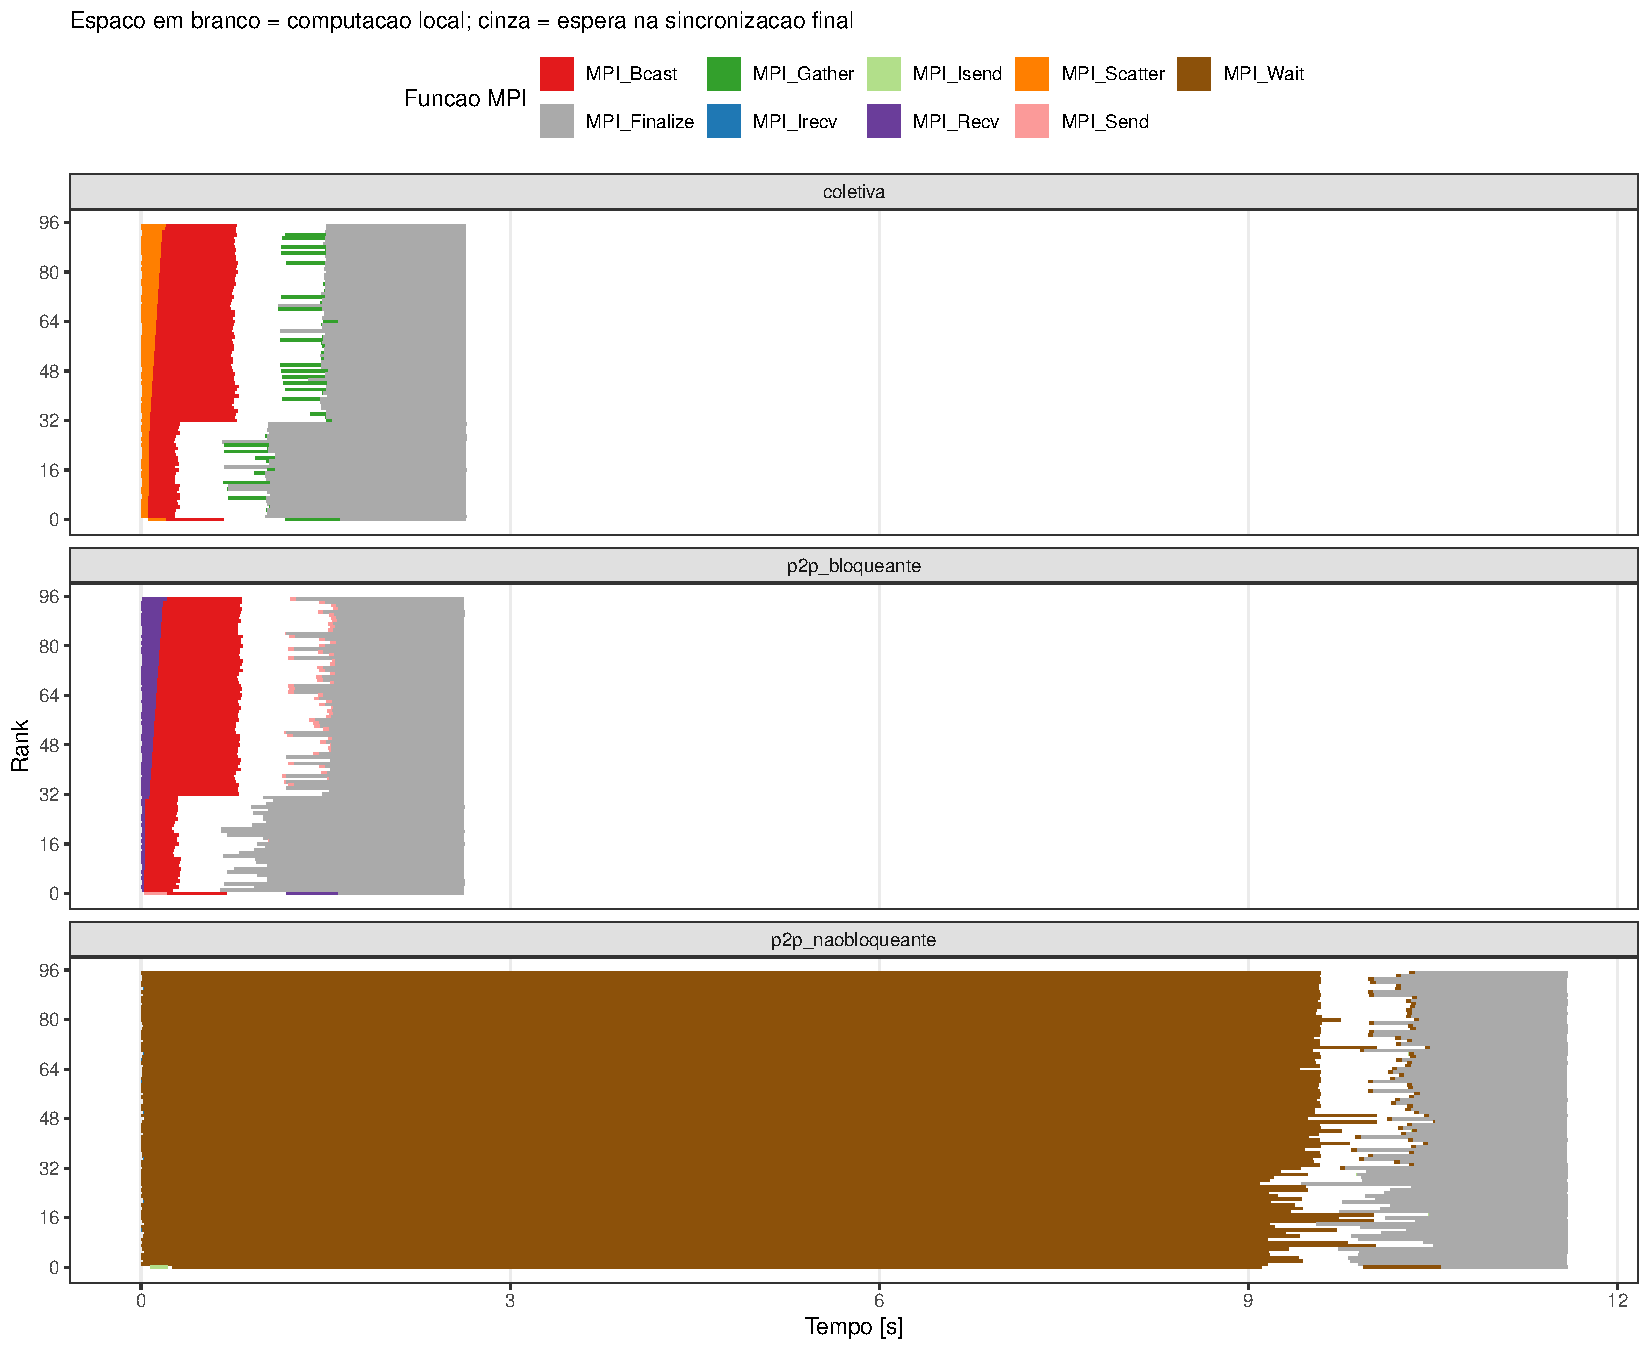
\includegraphics[width=0.8\textwidth]{imgs/gantt_geral.pdf}
\caption{Uma execução de cada versão (size=1500, 96 processos, 3 nós). Cada linha horizontal é um processo.}
\label{fig:gantt_geral}
\end{figure}

A leitura do quadro geral já resume o experimento: nas versões coletiva
e bloqueante a comunicação ocupa só o começo e o fim, e tudo termina em
cerca de 2.7s. Na versão não bloqueante quase todo o gráfico é marrom
(\texttt{MPI\_Wait}): os processos passam a maior parte dos
\textasciitilde10s de execução \textbf{esperando} dados chegarem.
Entender esse marrom é o ponto central da análise (seção seguinte).

Para ver as diferenças de semântica entre as versões, ampliamos os
primeiros 0.6s (fase de distribuição dos dados):

\begin{figure}[H]
\centering
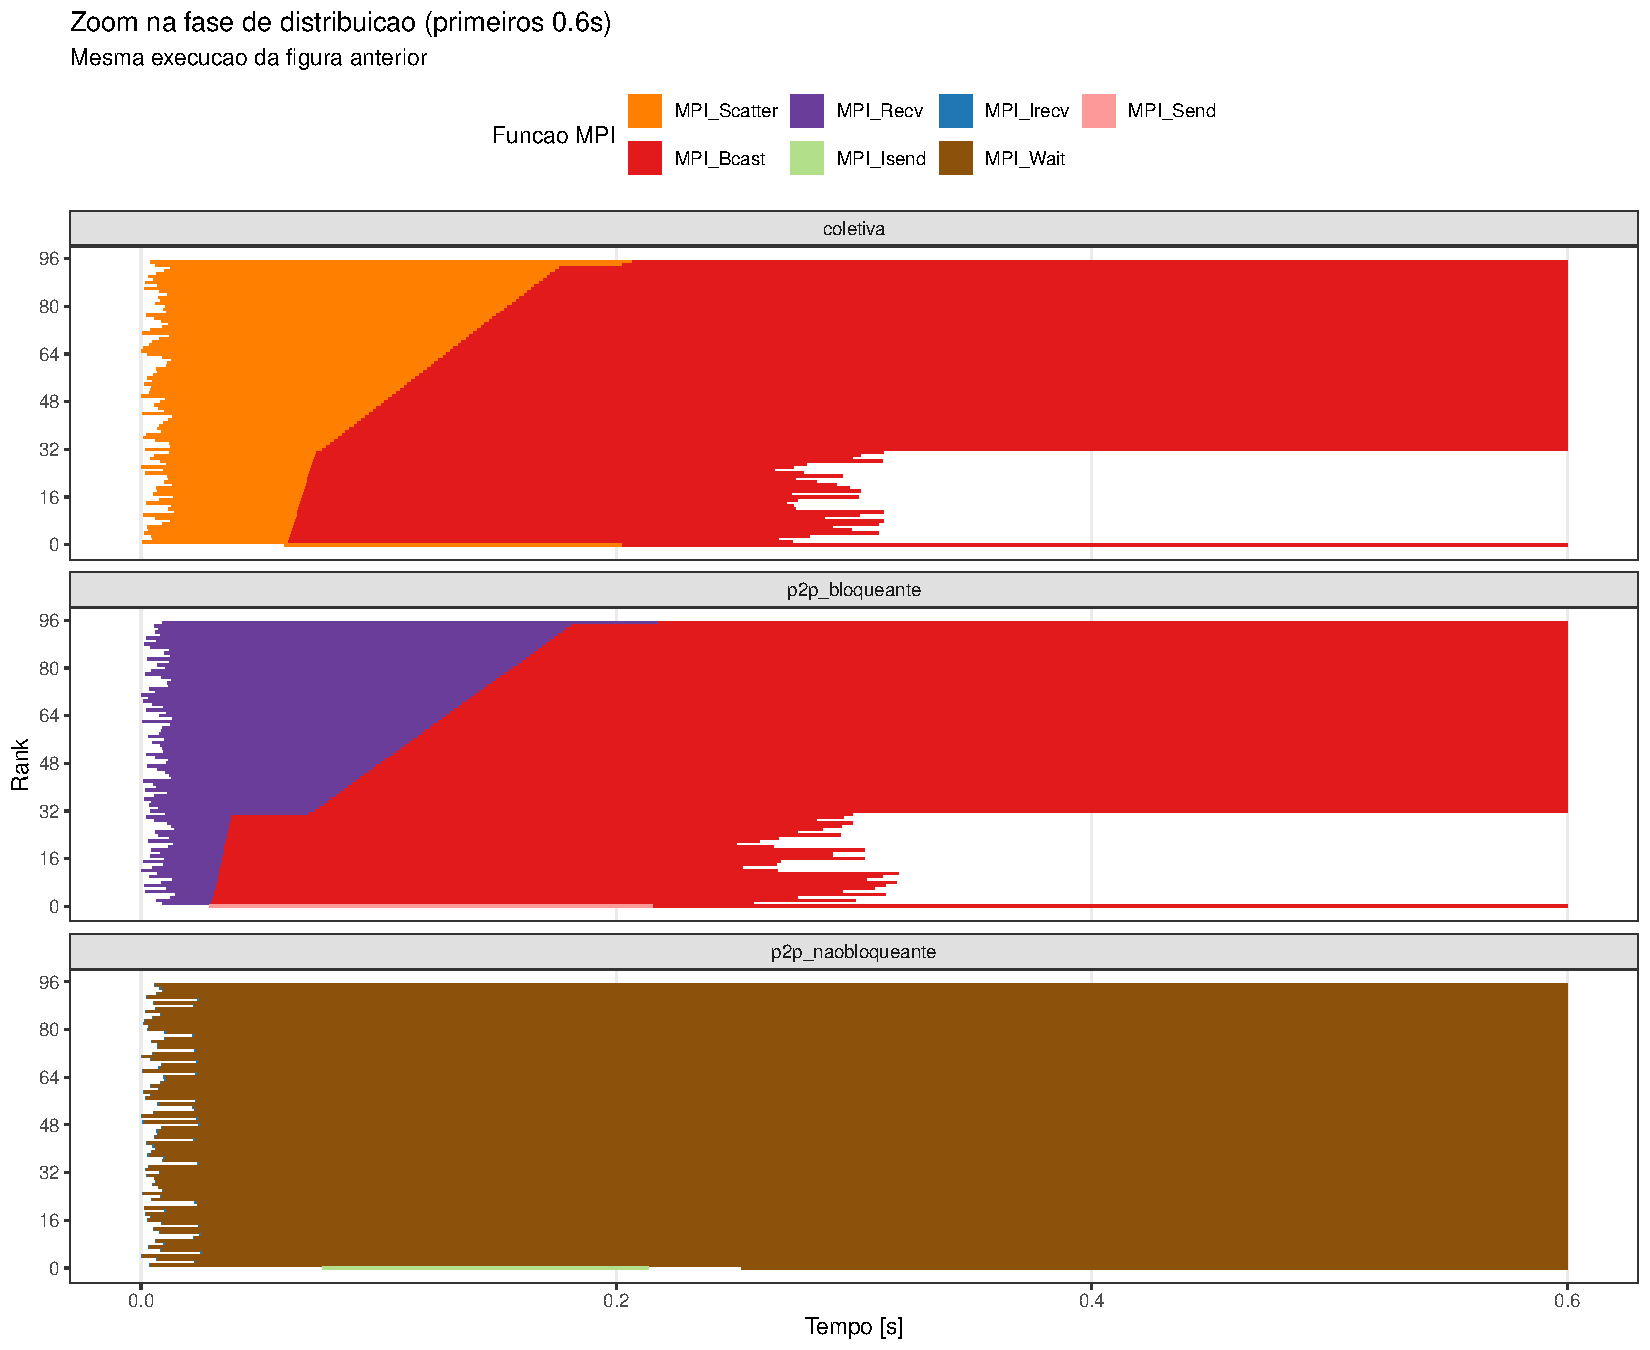
\includegraphics[width=0.8\textwidth]{imgs/gantt_dist.pdf}
\caption{Zoom nos primeiros 0.6s da mesma execução.}
\label{fig:gantt_dist}
\end{figure}

\begin{itemize}
\tightlist
\item
  \textbf{Coletiva}: todos entram juntos no \texttt{Scatter} (laranja) e
  depois no \texttt{Bcast} (vermelho). Note a fronteira de nó: os
  processos 0-31 (mesmo nó do mestre) saem do \texttt{Bcast} em
  \textasciitilde0.3s e começam a computar; os processos remotos só saem
  em \textasciitilde0.7s, porque receber B pela rede demora mais.
\item
  \textbf{Bloqueante}: os trabalhadores ficam parados no \texttt{Recv}
  (roxo) esperando sua vez, enquanto o mestre envia os 95 pedaços um por
  um -- por isso a borda roxa é diagonal: quanto maior o rank, mais
  tarde o dado chega. Depois, o mesmo \texttt{Bcast} da coletiva.
\item
  \textbf{Não bloqueante}: os \texttt{Irecv} retornam instantaneamente
  (mal aparecem) e a espera real acontece no \texttt{Wait} (marrom).
  Importante: o rastreador não registra o \texttt{MPI\_Ibcast} como um
  estado separado, então a espera pela matriz B também está dentro desse
  \texttt{Wait}.
\end{itemize}

\section{Tempo por operação MPI}\label{tempo-por-operauxe7uxe3o-mpi}

O gráfico abaixo decompõe o tempo total por função MPI para size=1500,
empilhando a contribuição de cada função. Permite ver de imediato qual
função domina o custo em cada versão e configuração.

\begin{figure}[H]
\centering
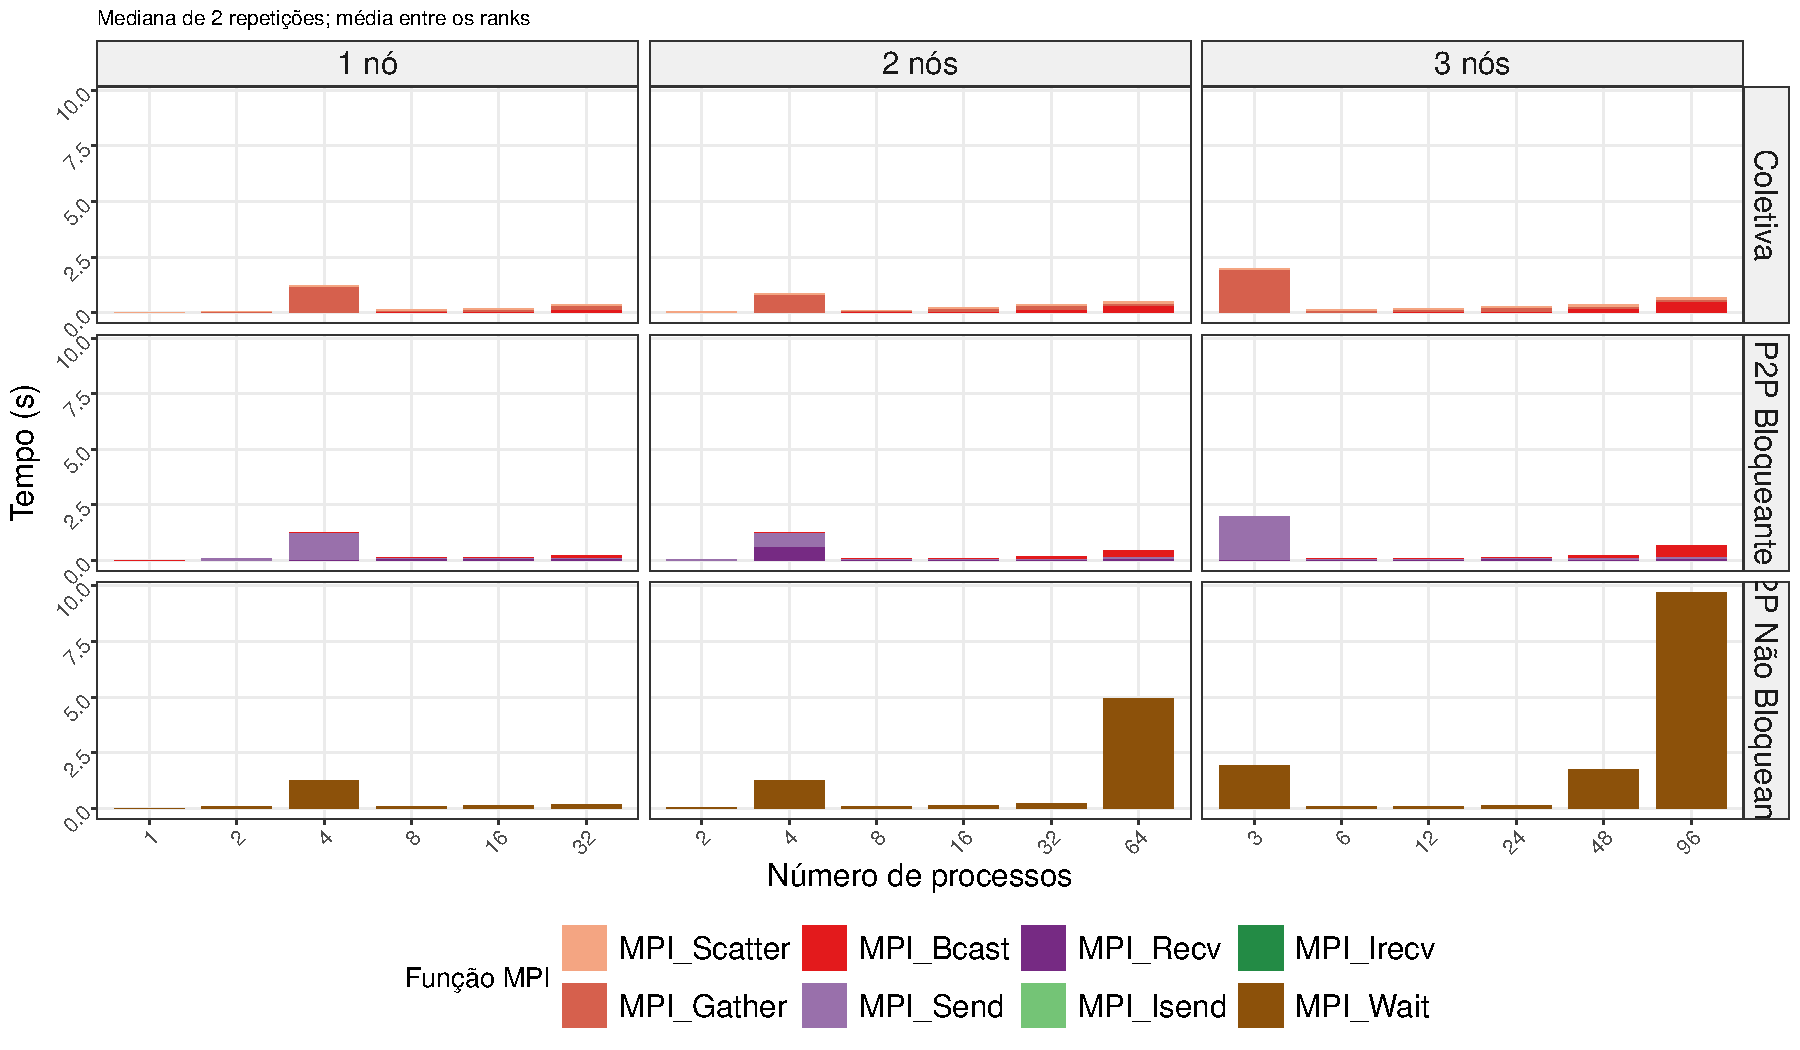
\includegraphics[width=0.8\textwidth]{imgs/plot_funcoes_stacked.pdf}
\caption{Tempo médio por processo em cada função MPI (size=1500, mediana de 2 repetições). Barras empilhadas por função.}
\label{fig:plot_funcoes_stacked}
\end{figure}

O gráfico seguinte isola a comparação central do experimento: o
\texttt{MPI\_Wait} da versão não bloqueante (que engloba a espera real
pela comunicação) versus o \texttt{MPI\_Bcast} das versões coletiva e
bloqueante (que fazem a mesma difusão de B, mas com algoritmo em
árvore).

\begin{figure}[H]
\centering
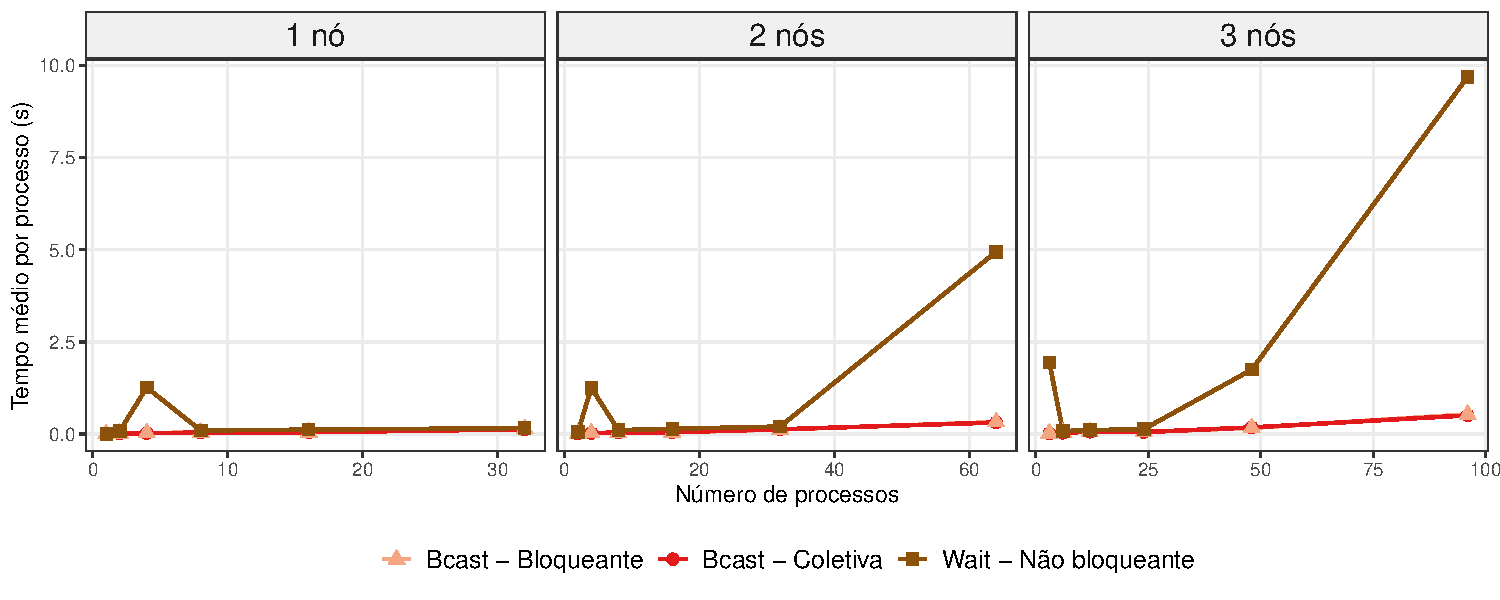
\includegraphics[width=0.8\textwidth]{imgs/plot_wait_vs_bcast.pdf}
\caption{MPI\_Wait (não bloqueante) vs MPI\_Bcast (coletiva e bloqueante) para size=1500. O colapso do Wait em múltiplos nós é a causa da lentidão da versão assíncrona.}
\label{fig:plot_wait_vs_bcast}
\end{figure}

A tabela abaixo mostra o tempo médio por processo em cada função
(mediana das 2 execuções), para size=1500 em 3 nós, nas duas maiores
quantidades de processos:

\begin{longtable}[]{@{}llll@{}}
\toprule\noalign{}
Função & Versão & 48 proc & 96 proc \\
\midrule\noalign{}
\endhead
\bottomrule\noalign{}
\endlastfoot
\texttt{MPI\_Wait} & não bloqueante & 1.75 s & \textbf{9.70 s} \\
\texttt{MPI\_Bcast} & coletiva & 0.18 s & 0.51 s \\
\texttt{MPI\_Bcast} & bloqueante & 0.17 s & 0.53 s \\
\texttt{MPI\_Gather} & coletiva & 0.11 s & 0.07 s \\
\texttt{MPI\_Scatter} & coletiva & 0.08 s & 0.10 s \\
\texttt{MPI\_Recv} & bloqueante & 0.06 s & 0.11 s \\
\texttt{MPI\_Send} & bloqueante & 0.03 s & 0.03 s \\
\texttt{MPI\_Isend} & não bloqueante & 0.002 s & 0.002 s \\
\texttt{MPI\_Irecv} & não bloqueante & 0.0005 s & 0.0005 s \\
\end{longtable}

Três coisas a notar:

\begin{enumerate}
\tightlist
\item
  Quase todas as operações custam décimos de segundo ou menos, mesmo com
  96 processos. A exceção é o \texttt{MPI\_Wait} da versão não
  bloqueante: 1.75s com 48 processos e 9.7s com 96 -- dobrar os
  processos multiplicou o custo por 5.5.
\item
  \texttt{Isend} e \texttt{Irecv} parecem "de graça" (milésimos de
  segundo), mas é ilusão: eles só iniciam a operação. O tempo que a
  comunicação realmente leva aparece depois, no \texttt{Wait}.
\item
  \texttt{MPI\_Bcast} custa praticamente o mesmo na coletiva e na
  bloqueante: as duas chamam exatamente a mesma função da biblioteca.
\end{enumerate}

Sobre como esses custos crescem: comparando execuções com o mesmo número
de processos em 1, 2 ou 3 nós, os tempos de \texttt{Scatter},
\texttt{Bcast} e \texttt{Recv} quase não mudam -- até \textasciitilde32
processos, o que importa é \textbf{quantos processos participam e quanto
dado trafega}, não quantos nós são usados. É acima de 32 processos (só
possível com 2 ou 3 nós) que os custos coletivos crescem mais rápido e o
\texttt{Wait} dispara.

\subsection{Tabela completa: todas as
combinações}\label{tabela-completa-todas-as-combinauxe7uxf5es}

A tabela abaixo traz o tempo médio por processo em cada função (em
segundos, mediana de 2 execuções) para \textbf{todas} as combinações de
tamanho, nós e processos. "Bcast (col)" e "Bcast (blq)" são o mesmo
\texttt{MPI\_Bcast} medido na versão coletiva e na bloqueante; "-"
indica função não chamada (com 1 processo não há trocas ponto a ponto);
"0.000" significa menos de 1 milissegundo.

\begin{longtable}[]{@{}llllllllllll@{}}
\toprule\noalign{}
size & nos & nproc & Scatter & Gather & Bcast (col) & Send & Recv &
Bcast (blq) & Isend & Irecv & Wait \\
\midrule\noalign{}
\endhead
\bottomrule\noalign{}
\endlastfoot
500 & 1 & 1 & 0.002 & 0.001 & 0.000 & - & - & 0.000 & - & - & 0.000 \\
500 & 1 & 2 & 0.005 & 0.002 & 0.001 & 0.001 & 0.004 & 0.002 & 0.001 &
0.000 & 0.007 \\
500 & 1 & 4 & 0.007 & 0.010 & 0.005 & 0.001 & 0.007 & 0.005 & 0.001 &
0.000 & 0.012 \\
500 & 1 & 8 & 0.005 & 0.002 & 0.004 & 0.000 & 0.010 & 0.005 & 0.000 &
0.000 & 0.011 \\
500 & 1 & 16 & 0.014 & 0.014 & 0.008 & 0.000 & 0.008 & 0.009 & 0.000 &
0.000 & 0.015 \\
500 & 1 & 32 & 0.014 & 0.008 & 0.050 & 0.001 & 0.012 & 0.035 & 0.001 &
0.000 & 0.043 \\
500 & 2 & 2 & 0.005 & 0.004 & 0.001 & 0.001 & 0.005 & 0.002 & 0.001 &
0.000 & 0.006 \\
500 & 2 & 4 & 0.007 & 0.004 & 0.004 & 0.001 & 0.008 & 0.005 & 0.001 &
0.000 & 0.009 \\
500 & 2 & 8 & 0.008 & 0.007 & 0.007 & 0.001 & 0.011 & 0.004 & 0.000 &
0.000 & 0.013 \\
500 & 2 & 16 & 0.011 & 0.011 & 0.007 & 0.001 & 0.015 & 0.008 & 0.000 &
0.000 & 0.022 \\
500 & 2 & 32 & 0.018 & 0.009 & 0.029 & 0.001 & 0.031 & 0.015 & 0.000 &
0.000 & 0.022 \\
500 & 2 & 64 & 0.057 & 0.005 & 0.072 & 0.001 & 0.035 & 0.045 & 0.001 &
0.001 & 0.488 \\
500 & 3 & 3 & 0.006 & 0.004 & 0.002 & 0.001 & 0.007 & 0.003 & 0.001 &
0.000 & 0.008 \\
500 & 3 & 6 & 0.008 & 0.026 & 0.006 & 0.001 & 0.010 & 0.007 & 0.000 &
0.000 & 0.011 \\
500 & 3 & 12 & 0.010 & 0.021 & 0.007 & 0.000 & 0.010 & 0.006 & 0.000 &
0.000 & 0.016 \\
500 & 3 & 24 & 0.007 & 0.006 & 0.011 & 0.001 & 0.013 & 0.012 & 0.000 &
0.000 & 0.021 \\
500 & 3 & 48 & 0.038 & 0.004 & 0.057 & 0.002 & 0.039 & 0.057 & 0.002 &
0.000 & 0.251 \\
500 & 3 & 96 & 0.044 & 0.004 & 0.125 & 0.001 & 0.033 & 0.097 & 0.001 &
0.001 & 1.080 \\
1000 & 1 & 1 & 0.005 & 0.003 & 0.000 & - & - & 0.000 & - & - & 0.000 \\
1000 & 1 & 2 & 0.015 & 0.008 & 0.005 & 0.003 & 0.023 & 0.008 & 0.002 &
0.000 & 0.016 \\
1000 & 1 & 4 & 0.019 & 0.081 & 0.012 & 0.002 & 0.025 & 0.016 & 0.002 &
0.000 & 0.088 \\
1000 & 1 & 8 & 0.024 & 0.077 & 0.018 & 0.001 & 0.021 & 0.018 & 0.001 &
0.000 & 0.044 \\
1000 & 1 & 16 & 0.019 & 0.072 & 0.022 & 0.001 & 0.037 & 0.023 & 0.001 &
0.000 & 0.056 \\
1000 & 1 & 32 & 0.033 & 0.059 & 0.079 & 0.002 & 0.033 & 0.070 & 0.001 &
0.000 & 0.097 \\
1000 & 2 & 2 & 0.015 & 0.011 & 0.005 & 0.002 & 0.014 & 0.007 & 0.002 &
0.000 & 0.016 \\
1000 & 2 & 4 & 0.020 & 0.124 & 0.013 & 0.002 & 0.016 & 0.014 & 0.002 &
0.000 & 0.038 \\
1000 & 2 & 8 & 0.019 & 0.081 & 0.019 & 0.001 & 0.034 & 0.019 & 0.001 &
0.000 & 0.031 \\
1000 & 2 & 16 & 0.025 & 0.036 & 0.024 & 0.001 & 0.046 & 0.026 & 0.001 &
0.000 & 0.088 \\
1000 & 2 & 32 & 0.031 & 0.047 & 0.105 & 0.001 & 0.039 & 0.036 & 0.001 &
0.000 & 0.069 \\
1000 & 2 & 64 & 0.046 & 0.023 & 0.146 & 0.013 & 0.077 & 0.167 & 0.002 &
0.001 & 2.204 \\
1000 & 3 & 3 & 0.018 & 0.011 & 0.008 & 0.002 & 0.016 & 0.010 & 0.002 &
0.000 & 0.022 \\
1000 & 3 & 6 & 0.018 & 0.064 & 0.016 & 0.002 & 0.025 & 0.021 & 0.002 &
0.000 & 0.046 \\
1000 & 3 & 12 & 0.023 & 0.049 & 0.032 & 0.002 & 0.031 & 0.037 & 0.001 &
0.000 & 0.051 \\
1000 & 3 & 24 & 0.027 & 0.049 & 0.028 & 0.001 & 0.033 & 0.026 & 0.001 &
0.000 & 0.060 \\
1000 & 3 & 48 & 0.045 & 0.029 & 0.092 & 0.016 & 0.064 & 0.119 & 0.001 &
0.000 & 0.793 \\
1000 & 3 & 96 & 0.065 & 0.020 & 0.248 & 0.001 & 0.072 & 0.271 & 0.002 &
0.001 & 4.361 \\
1500 & 1 & 1 & 0.010 & 0.006 & 0.000 & - & - & 0.000 & - & - & 0.000 \\
1500 & 1 & 2 & 0.030 & 0.034 & 0.010 & 0.052 & 0.023 & 0.014 & 0.003 &
0.000 & 0.084 \\
1500 & 1 & 4 & 0.051 & 1.167 & 0.023 & 1.196 & 0.043 & 0.026 & 0.003 &
0.000 & 1.261 \\
1500 & 1 & 8 & 0.035 & 0.057 & 0.038 & 0.002 & 0.085 & 0.041 & 0.002 &
0.000 & 0.096 \\
1500 & 1 & 16 & 0.050 & 0.097 & 0.046 & 0.002 & 0.082 & 0.048 & 0.002 &
0.000 & 0.119 \\
1500 & 1 & 32 & 0.052 & 0.216 & 0.128 & 0.002 & 0.079 & 0.138 & 0.002 &
0.000 & 0.160 \\
1500 & 2 & 2 & 0.030 & 0.019 & 0.010 & 0.024 & 0.022 & 0.014 & 0.003 &
0.000 & 0.047 \\
1500 & 2 & 4 & 0.038 & 0.813 & 0.027 & 0.605 & 0.620 & 0.026 & 0.003 &
0.000 & 1.253 \\
1500 & 2 & 8 & 0.034 & 0.046 & 0.039 & 0.002 & 0.066 & 0.040 & 0.002 &
0.000 & 0.105 \\
1500 & 2 & 16 & 0.052 & 0.133 & 0.048 & 0.001 & 0.063 & 0.044 & 0.002 &
0.000 & 0.141 \\
1500 & 2 & 32 & 0.066 & 0.202 & 0.127 & 0.002 & 0.059 & 0.122 & 0.003 &
0.000 & 0.203 \\
1500 & 2 & 64 & 0.106 & 0.100 & 0.312 & 0.021 & 0.107 & 0.323 & 0.002 &
0.001 & 4.945 \\
1500 & 3 & 3 & 0.036 & 1.936 & 0.017 & 1.948 & 0.031 & 0.022 & 0.003 &
0.000 & 1.939 \\
1500 & 3 & 6 & 0.038 & 0.066 & 0.033 & 0.003 & 0.061 & 0.035 & 0.003 &
0.000 & 0.079 \\
1500 & 3 & 12 & 0.051 & 0.103 & 0.061 & 0.002 & 0.053 & 0.059 & 0.002 &
0.000 & 0.105 \\
1500 & 3 & 24 & 0.052 & 0.181 & 0.052 & 0.001 & 0.088 & 0.053 & 0.001 &
0.000 & 0.131 \\
1500 & 3 & 48 & 0.076 & 0.113 & 0.178 & 0.025 & 0.060 & 0.166 & 0.002 &
0.000 & 1.748 \\
1500 & 3 & 96 & 0.103 & 0.073 & 0.506 & 0.025 & 0.109 & 0.533 & 0.002 &
0.001 & 9.696 \\
\end{longtable}

O que a tabela mostra, coluna a coluna:

\begin{itemize}
\tightlist
\item
  \textbf{Todas as funções bloqueantes ficam baratas em todas as
  combinações}: \texttt{Scatter}, \texttt{Gather}, \texttt{Bcast},
  \texttt{Send} e \texttt{Recv} raramente passam de 0.1-0.2s, mesmo com
  96 processos e matriz 1500. O custo cresce suavemente com o tamanho
  (mais bytes) e com o número de processos (mais participantes), mas
  nunca explode.
\item
  \textbf{A coluna \texttt{Wait} é a única que explode}, e de forma
  consistente nas três dimensões: cresce com o tamanho (com 64
  processos: 0.49s em size=500, 2.20s em 1000, 4.95s em 1500), cresce
  com os processos (em size=1500: 0.20s com 32, 1.75s com 48, 4.95s com
  64, 9.70s com 96) e só explode quando há mais de um nó -- em 1 nó o
  \texttt{Wait} fica sempre abaixo de 0.16s. São exatamente as três
  assinaturas do problema do \texttt{Ibcast} descrito na seção de
  investigação: mais bytes, mais destinos e rede no caminho.
\item
  Os valores altos isolados de \texttt{Gather=/=Send} em size=1500 com
  3-4 processos (\textasciitilde1.2-1.9s) não são custo de comunicação:
  são o mestre esperando trabalhadores que computam mais devagar (o
  desbalanceamento de memória citado na próxima seção) dentro da chamada
  de coleta.
\end{itemize}

\section{Tempo total de execução}\label{tempo-total-de-execuuxe7uxe3o}

Mediana das 2 execuções, size=1500 (os tamanhos menores mostram as
mesmas tendências).

O gráfico abaixo mostra o tempo total para todas as combinações de
tamanho de matriz, número de nós e número de processos. Cada painel
corresponde a um tamanho de matriz (linhas) e uma configuração de nós
(colunas); o eixo x está em escala logarítmica.

\begin{figure}[H]
\centering
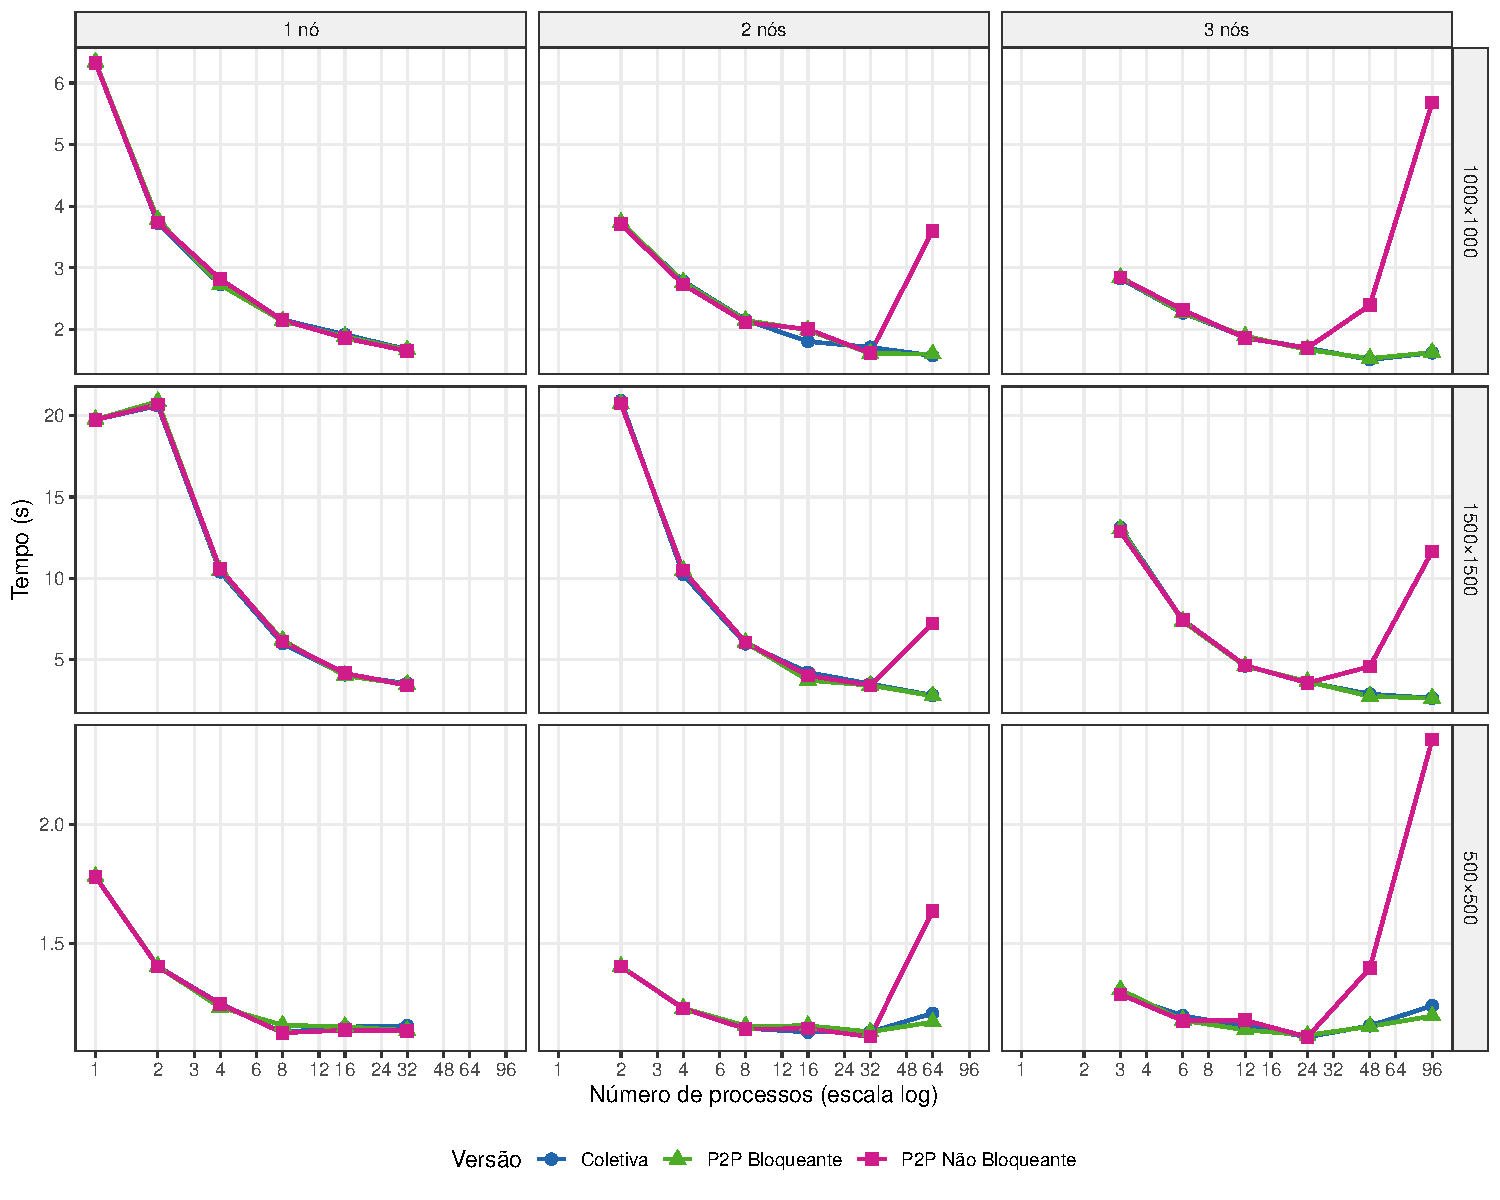
\includegraphics[width=0.8\textwidth]{imgs/plot_tempo_total.pdf}
\caption{Tempo total de execução (mediana de 2 repetições) para todas as combinações experimentais. Eixo x em escala log.}
\label{fig:plot_tempo_total}
\end{figure}

O gráfico de escalabilidade abaixo fixa o número de processos por nó e
varia o número de nós, isolando o efeito da comunicação inter-nó. As
barras de erro indicam o desvio padrão entre as 2 repetições.

\begin{figure}[H]
\centering
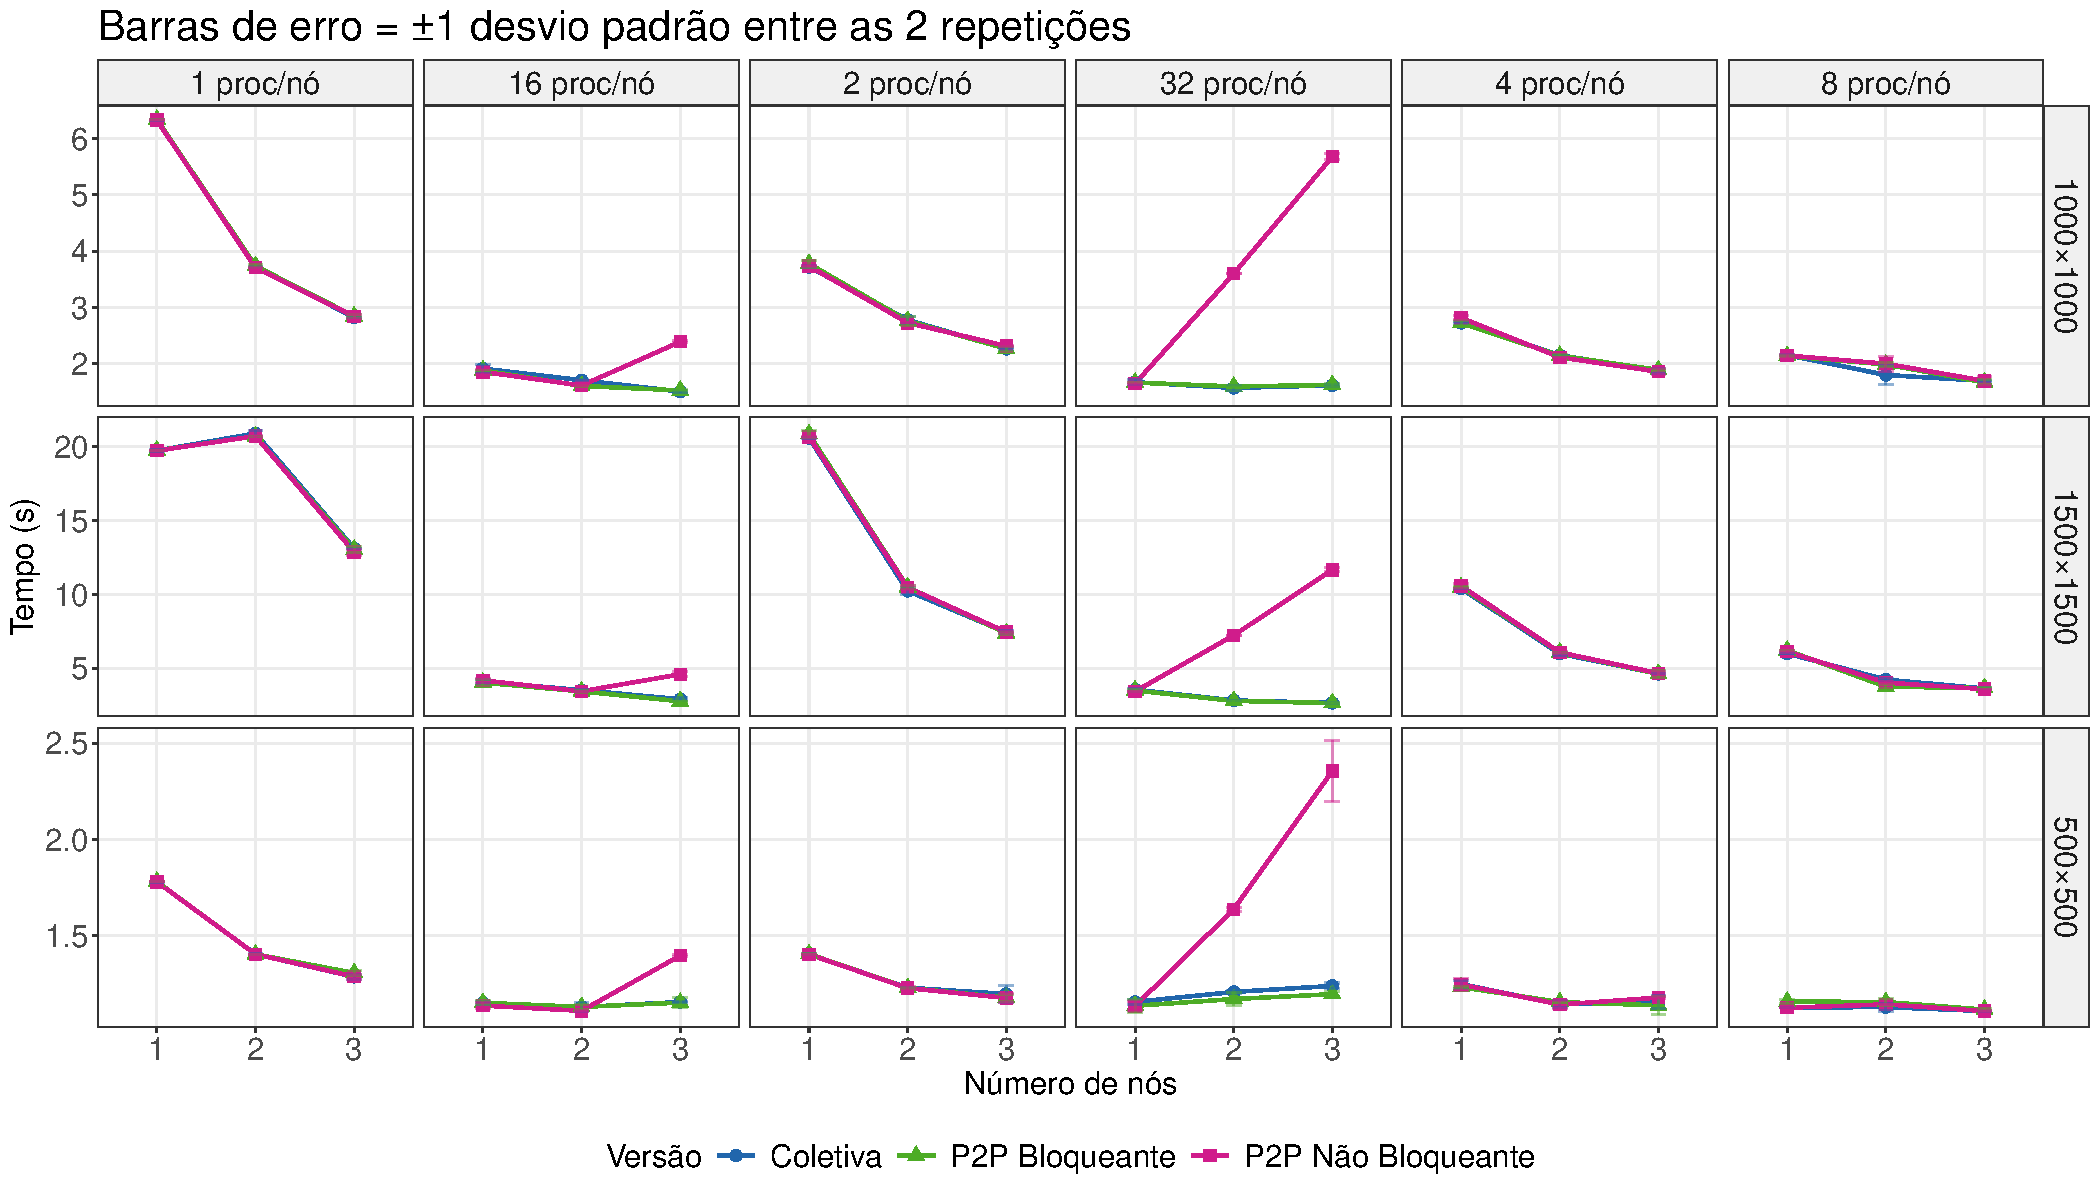
\includegraphics[width=0.8\textwidth]{imgs/plot_escalabilidade_nos.pdf}
\caption{Escalabilidade por número de nós com número de processos por nó fixo. Barras de erro = ±1 desvio padrão.}
\label{fig:plot_escalabilidade_nos}
\end{figure}

\begin{longtable}[]{@{}lllll@{}}
\toprule\noalign{}
Nós & nproc & coletiva & p2p bloq. & p2p não bloq. \\
\midrule\noalign{}
\endhead
\bottomrule\noalign{}
\endlastfoot
1 & 1 & 18.71 s & 18.72 s & 18.70 s \\
1 & 2 & 19.57 s & 19.83 s & 19.64 s \\
1 & 8 & 4.95 s & 5.15 s & 5.06 s \\
1 & 32 & 2.48 s & 2.41 s & 2.36 s \\
2 & 32 & 2.44 s & 2.37 s & 2.37 s \\
2 & 64 & 1.74 s & 1.72 s & \textbf{6.16 s} \\
3 & 48 & 1.83 s & 1.71 s & \textbf{3.53 s} \\
3 & 96 & 1.57 s & 1.58 s & \textbf{10.60 s} \\
\end{longtable}

O speedup de cada versão em relação à execução sequencial (1 processo, 1
nó) é mostrado abaixo em escala log×log. A linha tracejada cinza
representa o speedup ideal (linear). Valores abaixo dela indicam ganho
sub-linear; valores que caem abruptamente indicam overhead de
comunicação superando o ganho de paralelismo.

\begin{figure}[H]
\centering
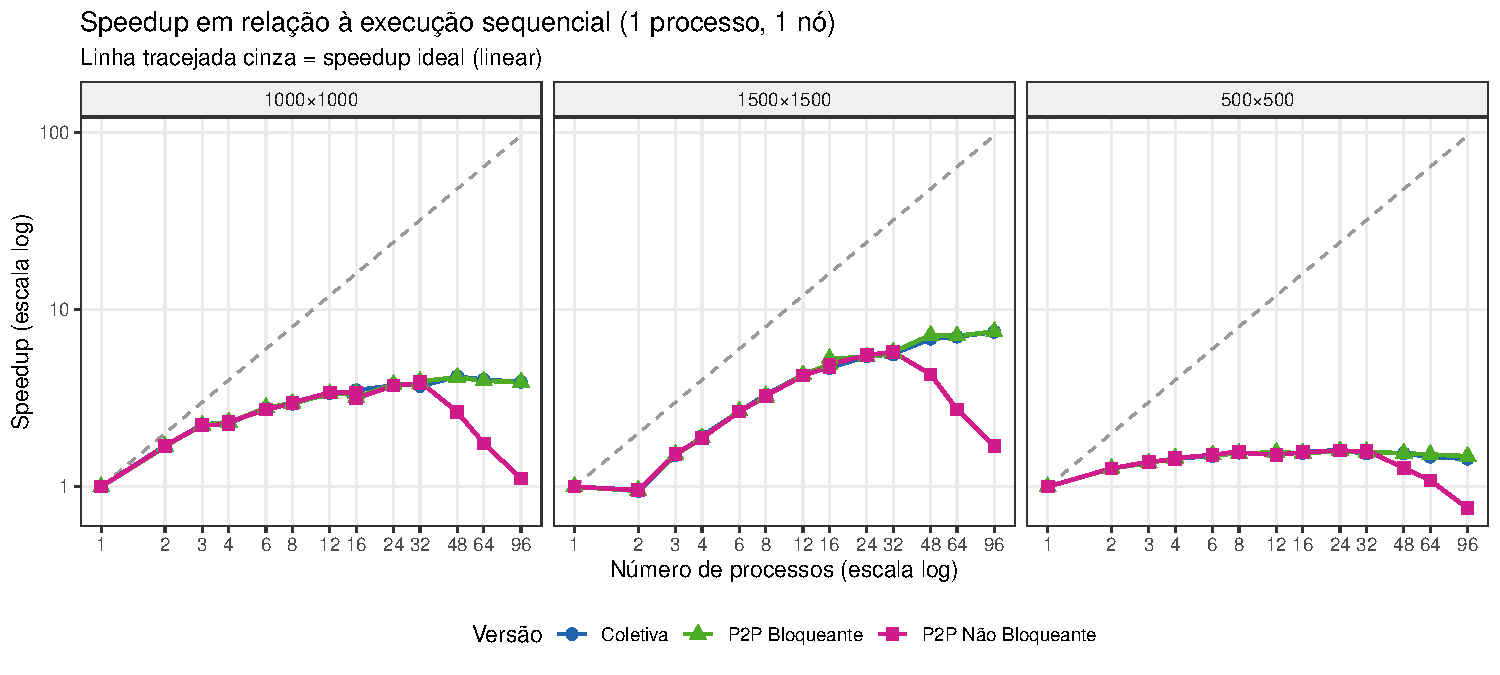
\includegraphics[width=0.8\textwidth]{imgs/plot_speedup.pdf}
\caption{Speedup em relação à execução com 1 processo. Escala log×log. Linha tracejada = speedup ideal.}
\label{fig:plot_speedup}
\end{figure}

Lendo a tabela de cima para baixo:

\begin{itemize}
\tightlist
\item
  \textbf{Em um nó, as três versões empatam} em todas as linhas: as
  diferenças ficam dentro da variabilidade entre repetições. Faz
  sentido: a multiplicação em si (o trecho branco do Gantt) leva
  segundos, enquanto toda a comunicação leva décimos de segundo. Quando
  a computação domina, o padrão de comunicação não importa.
\item
  Uma curiosidade: com 2 processos o tempo \emph{não cai} em relação a 1
  (18.7s -\textgreater{} 19.6s). Isso só acontece no tamanho 1500 -- nos
  tamanhos 500 e 1000 o tempo cai perfeitamente pela metade. Como o
  efeito é idêntico nas três versões, ele vem da máquina (disputa por
  memória/cache entre processos no mesmo nó, já que cada processo
  carrega uma cópia de B com 18MB) e não interfere na comparação entre
  os padrões.
\item
  \textbf{Com 2 e 3 nós, coletiva e bloqueante continuam melhorando} (o
  melhor tempo do experimento é 1.57s, com 96 processos), mas \textbf{a
  versão não bloqueante piora muito}: 6.16s com 64 processos e 10.60s
  com 96 -- quase 7x mais lenta que as outras duas.
\end{itemize}

\section{Investigando o colapso da versão não
bloqueante}\label{investigando-o-colapso-da-versuxe3o-nuxe3o-bloqueante}

Por que a versão assíncrona fica 7x mais lenta justamente na maior
configuração? O rastro permite responder passo a passo.

Cada trabalhador chama \texttt{MPI\_Wait} exatamente 3 vezes, nesta
ordem: (1) esperar as linhas de A chegarem, (2) esperar a matriz B do
\texttt{Ibcast}, (3) esperar o envio do resultado. Olhando um
trabalhador da execução com 96 processos, as durações dos 3
\texttt{Wait} são:

\begin{longtable}[]{@{}ll@{}}
\toprule\noalign{}
Espera & Duração \\
\midrule\noalign{}
\endhead
\bottomrule\noalign{}
\endlastfoot
(1) linhas de A (\texttt{Irecv}) & 0.07 s \\
(2) matriz B (\texttt{Ibcast}) & \textbf{9.1 s} \\
(3) resultado (\texttt{Isend}) & \textasciitilde0 s \\
\end{longtable}

Ou seja: praticamente todo o tempo de \texttt{Wait} é \textbf{espera
pela matriz B}. A mesma difusão de B, quando feita com o
\texttt{MPI\_Bcast} bloqueante, custa 0.5s (tabela da seção anterior). A
diferença é a implementação: o \texttt{Bcast} bloqueante usa um
algoritmo em árvore (o dado se propaga em paralelo, em O(log P) etapas),
enquanto o \texttt{Ibcast} não bloqueante da biblioteca usa um esquema
muito menos eficiente. Uma conta simples sustenta essa leitura: se o
mestre enviasse B (18MB) individualmente para cada um dos 64 processos
remotos por uma rede de 1Gb/s, levaria 18MB x 64 / 125MB/s
\textasciitilde{} 9.8s -- exatamente a ordem do que medimos. Em 1 nó não
há rede envolvida (memória compartilhada), por isso o problema só
aparece em execuções multi-nó.

A lição não é "assíncrono é lento", e sim dupla: (1) trocar chamadas
bloqueantes por não bloqueantes \emph{sem computar nada entre o início e
o} \emph{\texttt{Wait}} apenas move a espera de lugar -- o algoritmo
aqui não sobrepõe computação e comunicação; e (2) as versões não
bloqueantes das coletivas podem ter implementação bem pior que as
bloqueantes, e isso só aparece quando a comunicação cruza a rede.

\section{Conclusão}\label{conclusuxe3o}

\begin{itemize}
\tightlist
\item
  Enquanto a computação domina (execuções em 1 nó), o padrão de
  comunicação é indiferente -- e a coletiva vence pela simplicidade do
  código.
\item
  Em múltiplos nós, coletiva e bloqueante escalam bem; a não bloqueante
  colapsa por causa do \texttt{MPI\_Ibcast}, cuja implementação não usa
  a árvore otimizada do \texttt{Bcast} bloqueante.
\item
  Comunicação assíncrona só compensa se o algoritmo computa enquanto
  espera. Sem essa sobreposição, ela no melhor caso empata e no pior
  caso perde por detalhes de implementação.
\end{itemize}

Para este algoritmo, a versão com \textbf{operações coletivas
(bloqueantes) é a preferível}: desempenho igual ou melhor em todos os
cenários, código mais simples e escalabilidade robusta.

\section{Referências}\label{referuxeancias}

Alguns experimentos deste trabalho utilizaram os recursos da
infraestrutura PCAD, \url{http://pcad.inf.ufrgs.br}, no INF/UFRGS.
